\documentclass{standalone}
\usepackage{ tikz }
\usetikzlibrary{shapes}
\usetikzlibrary{plotmarks}
\usepackage{ xparse }
\usepackage{../../../macros}

\begin{document}
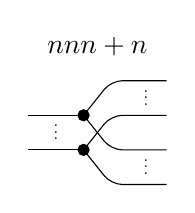
\begin{tikzpicture}[yscale=-1,x=1em,y=1.25em]
        
    \node at (1.5,-2) {$\morph{\ccopy{n}}{n}{n + n}$};

    \draw (-1,0) -- (1,0);
    \node at (0,0.35) {\scalebox{0.6}{$\vdots$}};
    \draw (-1,1) -- (1,1);

    \filldraw (1,0) circle (2pt);
    \filldraw (1,1) circle (2pt);

    \draw [rounded corners] (1,0) -- (2,-1) -- (4,-1);
    \draw [rounded corners] (1,1) -- (2,0) -- (4,0);
    \draw [rounded corners] (1,0) -- (2,1) -- (4,1);
    \draw [rounded corners] (1,1) -- (2,2) -- (4,2);

    \node at (3.25,1.35) {\scalebox{0.6}{$\vdots$}};
    \node at (3.25,-0.65) {\scalebox{0.6}{$\vdots$}};

\end{tikzpicture}
\end{document}